\documentclass[a4paper]{article}
\usepackage{german}
\usepackage[utf8]{inputenc}

\usepackage{pgfplots}
\usepackage{pgfplots.assert}

\usetikzlibrary{intersections}

\begin{document}

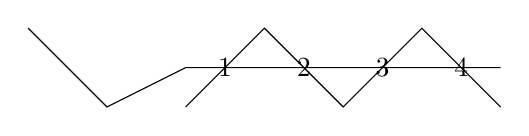
\begin{tikzpicture}
%\tracingcommands=2\tracingmacros=2
	\draw[name path=A] plot coordinates {
		  (2,0) (3,1) (4,0) (5,1) (6,0)
	};

	\draw[name path=B] plot coordinates {
		(0,1) (1,0) (2,0.5) (6,0.5)
	};

	\pgfintersectionofpaths%
		{%
			\expandafter\pgfsetpath\csname tikz@intersect@path@name@A\endcsname%
		}%
		{%
			\expandafter\pgfsetpath\csname tikz@intersect@path@name@B\endcsname%
		}%

	\pgfplotsassertequalstok{4}{\pgfintersectionsolutions}{}

	\foreach \i in {1,2,...,\pgfintersectionsolutions} {%
		\begingroup
		\pgftransformshift{\pgfpointintersectionsolution{\i}}%
		\node at (0,0) {\i};
		\endgroup
	}%

	\pgfintersectiongetsolutionsegmentindices{1}\Aindex\Bindex
	\pgfplotsassertequalstok{0}{\Aindex}{solution 1 path A}
	\pgfplotsassertequalstok{2}{\Bindex}{solution 1 path B}
	
	\pgfintersectiongetsolutionsegmentindices{2}\Aindex\Bindex
	\pgfplotsassertequalstok{1}{\Aindex}{solution 2 path A}
	\pgfplotsassertequalstok{2}{\Bindex}{solution 2 path B}

	\pgfintersectiongetsolutionsegmentindices{3}\Aindex\Bindex
	\pgfplotsassertequalstok{2}{\Aindex}{solution 3 path A}
	\pgfplotsassertequalstok{2}{\Bindex}{solution 3 path B}

	\pgfintersectiongetsolutionsegmentindices{4}\Aindex\Bindex
	\pgfplotsassertequalstok{3}{\Aindex}{solution 4 path A}
	\pgfplotsassertequalstok{2}{\Bindex}{solution 4 path B}
\end{tikzpicture}
\end{document}

